\documentclass[tikz]{standalone}
\usepackage{pgfplots}
\pgfplotsset{compat=1.15}
\usepackage{mathrsfs}
\usetikzlibrary{arrows,calc}
\usepackage{tkz-euclide}

\pagestyle{empty}

\definecolor{AngleClr}{rgb}{0,0.39215686274509803,0}
\definecolor{ShapeClr}{rgb}{0.6,0.2,0}

\begin{document}

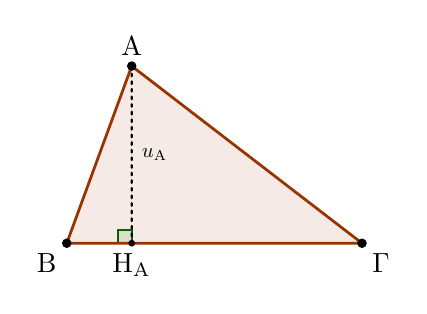
\begin{tikzpicture}[scale=.75]
\tkzSetUpLine[line width=1pt,color=black]
\tkzSetUpPoint[fill=black]


\tkzDefPoints{0/0/B,1.1/3/A,5/0/C}

\tkzDefTriangleCenter[ortho](A,B,C)
\tkzGetPoint{H}

\tkzDefPointBy[projection=onto B--C](H)\tkzGetPoint{HA}

\tkzFillPolygon[fill=ShapeClr,fill opacity=0.1](A,B,C)

\tkzMarkRightAngle[line width=0.75pt, size=.225,color=AngleClr,fill=AngleClr,fill opacity=0.1](H,HA,B)
\tkzDrawPolygon[color=ShapeClr](A,B,C)

\tkzDrawSegment[line width=0.75pt,color=black,dashed,dash pattern=on 1pt off 1.75pt](A,HA)


\tkzDrawPoints[size=3](A,B,C)
\tkzDrawPoints[size=2](HA)
\tkzLabelPoint[above](A){$\rm A$}
\tkzLabelPoint[below left](B){$\rm B$}
\tkzLabelPoint[below right](C){$\rm \Gamma$}
\tkzLabelPoint[below](HA){$\rm H_A$}

\tkzLabelSegment[right](A,HA){\scalebox{0.75}{$u_{\rm A}$}}

\end{tikzpicture}

\end{document}
